\documentclass[]{beamer}
\usepackage[T1]{fontenc}
\usepackage[utf8]{inputenc}
\usepackage{lmodern}
\usepackage[italian]{babel}
\usepackage{mathrsfs}
\usepackage{cancel}

\title{Il campo elettrico}
\author{\texorpdfstring{Mattia Cozzi\newline\href{mailto:cozzimattia@gmail.com}{\texttt{cozzimattia@gmail.com}}}{Mattia Cozzi}}
\date{a.s.~2023/2024}

%\documentclass[handout]{beamer}     %usare questa classe per generare l'handout
%\usepackage{pgfpages}   %per mostrare più quadri nella stessa pagina
%\pgfpagesuselayout{4 on 1}[a4paper,border shrink=5mm,landscape]
\usetheme{Singapore}
%\useoutertheme[left]{sidebar} %elementi intorno alle diapositive
\setbeamercovered{dynamic} %modifica l'aspetto del testo grigetto delle diapositive future. Argomenti: invisible/transparent/dynamic
\usecolortheme{orchid}
%COLORE PRINCIPALE
\definecolor{marroncino}{RGB}{156, 26, 0} % UBC Blue (primary)
\setbeamercolor{structure}{fg=marroncino} % itemize, enumerate, etc


\theoremstyle{plain}
\newtheorem{teorema}{Teorema}

\usepackage{tikz}
\usepackage{circuitikz}

\usepackage{pgf,pgfplots,graphicx}
\usetikzlibrary{angles,quotes,arrows,shapes,decorations.markings}
\pgfplotsset{compat=1.15}
\usepgfplotslibrary{units,fillbetween} % to add units easily to axis

\newcommand{\fem}{f_{em}}

\def\angolo[#1](#2)(#3:#4:#5)% Syntax: [draw options] (center) (initial angle:final angle:radius)
    { \draw[#1] ($(#2)+({#5*cos(#3)},{#5*sin(#3)})$) arc (#3:#4:#5); }


\begin{document}

\begin{frame}
  \titlepage
\end{frame}





\begin{frame}
\frametitle{Contenuti}
\tableofcontents
\end{frame}


\section{Concetto}

\begin{frame}
\frametitle{Il concetto di campo (1)}
La forza tra due cariche è una \emph{forza a distanza}, come quella di gravità che si esercita tra due masse.

~

Come possono due corpi non in contatto interagire tra loro?\pause

~

Questa difficoltà viene superata ipotizzando che:
\begin{itemize}
  \item la presenza di una carica (massa) in un certo punto dello spazio \alert<2>{modifica le caratteristiche dello spazio} circostante;\pause
  \item un'altra carica (massa) posta nello spazio circostante \alert<3>{risente di una forza dovuta alle nuove proprietà dello spazio}.
\end{itemize}
\end{frame}


\begin{frame}
\frametitle{Il concetto di campo (2)}

\begin{figure}
\begin{tikzpicture}[scale=0.5]
\node [above,red] at (6,.1) {$ q_p $};
\draw [red, ultra thick,fill=red] (6,0) circle [radius=.1];\pause
\visible<2->{\draw [->, thick] (6,0) -- (10,0);
\node [above] at (8,0) {$ \vec{F} $};
\node [above,red] at (0,.7) {$ Q_S $};
\draw [red, ultra thick,fill=red] (0,0) circle [radius=.7];
\draw [red, ultra thick,fill=red] (6,0) circle [radius=.1];}
\end{tikzpicture}
\end{figure}
Poniamo una \emph<1>{carica di prova} (positiva e sufficientemente piccola da non modificare il sistema fisico in esame) $ q_p $ in un punto dello spazio.

~

\visible<2->{Se introduciamo una \emph<2>{carica sorgente} positiva $ Q_S $ allora \alert{$ q_p $ inizierà a sentire una forza $ \vec{F} $} dovuta alle nuove proprietà del punto in cui si trova.}
\end{frame}


\section{$ \vec{E} $}

\begin{frame}
\frametitle{Campo vettoriale}
Il campo elettrico (e quello gravitazionale) sono \emph{campi vettoriali}.

\begin{block}{Definizione}
\begin{columns}
\begin{column}{0.4\textwidth}
Un campo vettoriale è una funzione che ad ogni punto dello spazio associa un vettore forza.
\end{column}
\begin{column}{0.4\textwidth}
\begin{figure}
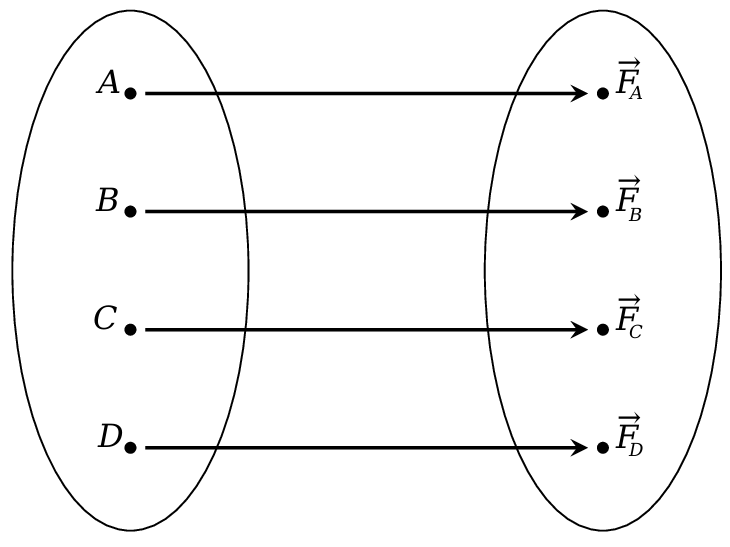
\includegraphics[width=.9\columnwidth]{img/funzionecampo.png}
\end{figure}
\end{column}
\end{columns}
\end{block}

Il vettore forza viene ottenuto con la legge di Coulomb o con quella di gravitazione universale.
\end{frame}


\begin{frame}
\frametitle{Il vettore campo elettrico}
\begin{figure}
\begin{tikzpicture}[scale=0.2]
\node [above,red] at (6,.1) {$ q_p $};
\draw [->, thick] (6,0) -- (10,0);
\node [above] at (8,0) {$ \vec{F} $};
\node [above,red] at (0,.7) {$ Q_S $};
\draw [red, ultra thick,fill=red] (0,0) circle [radius=.7];
\draw [red, ultra thick,fill=red] (6,0) circle [radius=.1];
\end{tikzpicture}
\end{figure}
Usando la nostra carica di prova $ q_p $ definiamo, per ogni punto dello spazio, il \alert{vettore campo elettrico}:

\begin{center}
\colorbox{marroncino!30}{$ \vec{E} = \dfrac{\vec{F}}{q_p} $}~~~~~~~~$ \left[\dfrac{N}{C}\right] $
\end{center}\pause
Notiamo che, in ogni punto dello spazio, \alert{$ \vec{E} $ è un vettore}:
\begin{itemize}
  \item con la stessa direzione e lo stesso verso di $ \vec{F} $;\pause
  \item con modulo pari a $ E = \dfrac{F}{q_p} $.
\end{itemize}
\end{frame}



\begin{frame}
\frametitle{Confronto con la forza peso}
Sappiamo che un corpo, nello spazio intorno ad un pianeta od una stella, è immerso in un \alert<1>{campo gravitazionale}.\pause

~

Subisce pertanto una forza, la \alert<2-3>{forza peso}, la cui intensità dipende dalla distanza dal pianeta:
\begin{center}
$ \vec{P} = m_p\vec{g} \pause ~~~~~\Longrightarrow~~~~~ $\colorbox{marroncino!30}{$ \vec{g} = \dfrac{\vec{P}}{m_p} $}\pause
\end{center}
Il valore di $ g $ (analogo di $ E $) indica \alert{l'intensità del campo gravitazionale} (elettrico) in una certa zona dello spazio.
\end{frame}







\begin{frame}
\frametitle{Esercizio}

  \begin{exampleblock}{Forza subita da una carica immersa in un campo elettrico}
{\small Una carica $ q = - 3,0 \, nC $ si trova in una zona di spazio interessata da un campo elettrico verso destra di $ 12,0 \, \frac{N}{C} $. A quale forza è soggetta?}
\end{exampleblock}
  \pause
  Invertiamo la definizione di campo elettrico:
  \begin{center}
  $ \vec{E} = \dfrac{\vec{F}}{q} \quad\quad \Longrightarrow \quad\quad \vec{F}=q\vec{E} $
  \end{center}\pause
  La carica sarà soggetta ad una forza di modulo:
  \begin{center}
  $ F = qE = - 3,0 \times 10^{-9} \, C \cdot 12,0 \, \dfrac{N}{C} = - 3,6 \times 10^{-8} \, N $
  \end{center}\pause
Il segno ``$ - $'' indica che la forza ha verso opposto al campo e sarà pertanto rivolta verso sinistra.

\end{frame}

\section{Sorgente}

\begin{frame}
\frametitle{Campo di una carica puntiforme}
In ogni punto dello spazio, possiamo calcolare il valore del campo elettrico generato da una carica sorgente $ Q_S $:
\begin{center}
$ E = \dfrac{F}{q_p} = \dfrac{k_0 \dfrac{Q_S \cancel{q_p}}{r^2}}{\cancel{q_p}} = k_0 \dfrac{Q_S }{r^2} $
\end{center}\pause
In un punto a distanza $ r $, una carica $ Q_S $ genera un campo di intensità:
\begin{center}
\colorbox{marroncino!30}{$ E = k_0 \dfrac{Q_S}{r^2} $}
\end{center}
\end{frame}


\begin{frame}
\frametitle{Verso del campo elettrico}
I vettori campo elettrico, essendo stati definiti attraverso la carica di prova positiva $ q_p $, saranno:
\begin{itemize}
  \item diretti verso l'esterno per cariche positive;
  \item diretti verso l'interno per cariche negative.
\end{itemize}
\begin{figure}
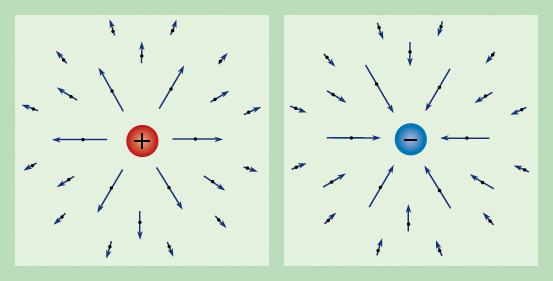
\includegraphics[width=.6\columnwidth]{img/vettoricampoelettrico.jpg}
\end{figure}
\end{frame}


\begin{frame}
\frametitle{Esercizio}

  \begin{exampleblock}{Calcolo della carica sorgente}
{\small Nel vuoto, ad una distanza di $ 7,4 \, cm $ da una carica $ Q $, si misura un campo elettrico di valore $ 9,2 \times 10^{4} \, \frac{N}{C} $ rivolto verso la carica. Quanto vale $ Q $?}
\end{exampleblock}
  \pause
  Poiché il campo è rivolto verso la carica, allora $ Q $ è negativa.{\pause} Dalla formula precedente inoltre otteniamo:
  \begin{center}
  $ Q = \dfrac{Er^2}{k_0} $
  \end{center}\pause
Eseguendo i calcoli:
  \begin{center}
  $ Q = \dfrac{ \left( -9,2 \times 10^4 \, \frac{N}{C}\right) \cdot ( 7,4 \times 10^{-2} \, m)^2 }{8,99 \times10^9 \, \frac{Nm^2}{C^2}} = - 5,6 \times 10^{-8} \, C $
  \end{center}
\end{frame}




\begin{frame}
\frametitle{Sovrapposizione}
\begin{block}{Principio di sovrapposizione}
Il campo totale che agisce in un punto $ P $ dello spazio è uguale alla \alert{somma vettoriale} dei singoli campi che agiscono in $ P $.
\end{block}
\begin{figure}
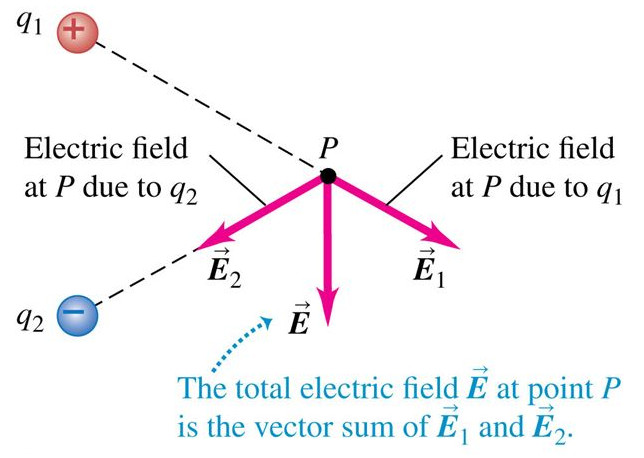
\includegraphics[width=.5\columnwidth]{img/sovrapposizionecampo.jpg}
\end{figure}
\end{frame}


\section{Linee}


\begin{frame}
\frametitle{Le linee del campo elettrico}

\begin{columns}
\begin{column}{0.6\textwidth}
Un campo elettrico è costituito da infiniti vettori. Per visualizzare un campo introduciamo le \emph{linee del campo elettrico}, che saranno:
\begin{itemize}
  \item uscenti da cariche positive, entranti nelle negative;
  \item tangenti in ogni punto dello spazio al vettore campo elettrico;
  \item più dense dove il campo è più intenso.
\end{itemize}
\end{column}
\begin{column}{0.3\textwidth}
\begin{figure}
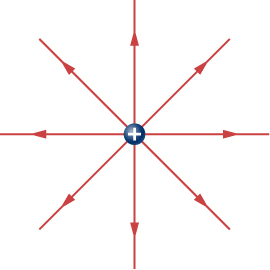
\includegraphics[width=.8\columnwidth]{img/campoelettrico1.jpg}
\end{figure}
\end{column}
\end{columns}
\end{frame}






\begin{frame}
\frametitle{Sovrapposizione di campi}
Sovrapponendo diversi campi tra loro possiamo ottenere diverse configurazioni delle linee di campo:
\begin{columns}
\begin{column}{0.3\textwidth}
\begin{figure}
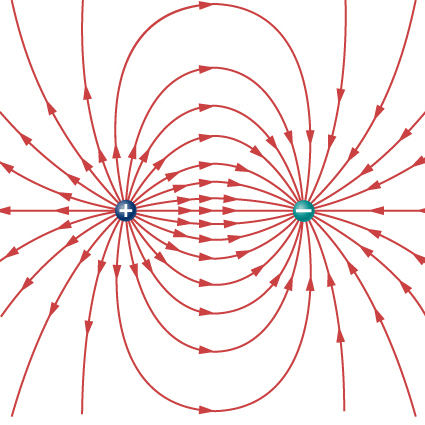
\includegraphics[width=\columnwidth]{img/campoelettrico2.jpg}
\end{figure}
\end{column}
\begin{column}{0.3\textwidth}
\begin{figure}
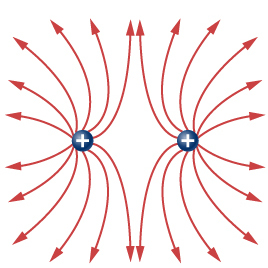
\includegraphics[width=\columnwidth]{img/campoelettrico3.jpg}
\end{figure}
\end{column}
\begin{column}{0.3\textwidth}
\begin{figure}
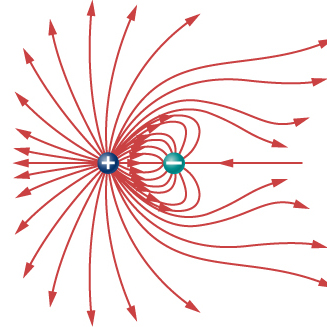
\includegraphics[width=\columnwidth]{img/campoelettrico4.jpg}
\end{figure}
\end{column}
\end{columns}
\end{frame}

\section{Flusso}


\begin{frame}
\frametitle{Prodotto scalare}
Per poter comprendere il concetto di ``flusso di un campo'' dobbiamo ricordare il \alert<1>{prodotto scalare tra due vettori $ \vec{a} $ e $ \vec{b} $}, che si calcola come:
  \begin{center}
  $ \vec{a} \cdot \vec{b} = a b \cos\theta $
  \end{center}
  con $ \theta $ angolo tra i due vettori.\\\pause~\\
  Intuitivamente, il prodotto scalare permette di valutare ``quanto del vettore $ \vec{a} $ giace sul vettore $ \vec{b} $''.
\end{frame}


\begin{frame}
\frametitle{Vettore superficie}
\visible<1->{Introduciamo, per utilizzarlo poi nella definizione di flusso, il \emph{vettore superficie}. Data una superficie piana $ S $, esso ha:}
  \begin{itemize}
    \item \visible<2->{direzione perpendicolare a $ S $;}
    \item \visible<3->{modulo pari a $ S $.} 
  \end{itemize}
  
  \begin{figure}
\begin{tikzpicture}
\visible<1->{\fill[fill=red!20] (0,0) -- (4,0) -- (3,-1) -- (-1,-1) -- cycle;
\node [right,thick] at (2.5,0) {$ S $};}
\visible<2->{\draw [dashed] (1.5,-.5) -- (1.5,2.5);
\draw [dotted] (1.5,-1) -- (1.5,-.5);
\draw [dashed] (1.5,-1) -- (1.5,-1.5);}
\visible<3->{\node [right,blue,thick] at (1.5,1) {$ \vec{S} $};
\draw [->,blue,thick] (1.5,-.5) -- (1.5,2);}
\end{tikzpicture}
\end{figure}

\end{frame}


\begin{frame}
  \frametitle{Flusso del campo elettrico}
Il flusso del campo elettrico è definito come il prodotto scalare tra il campo elettrico $ \vec{E} $ che attraversa la superficie $ S $ e il vettore superficie $ \vec{S} $ definito sopra.
\begin{center}
   \colorbox{marroncino!30}{$ \Phi_{S}(\vec{E}) = \vec{E} \cdot \vec{S} = ES\cos\theta $}
\end{center}
\begin{figure}
\begin{tikzpicture}
\fill[fill=red!20] (0,0) -- (4,0) -- (3,-1) -- (-1,-1) -- cycle;
\angolo[black](1.5,-.5)(52:90:.8)
\node [left,thick] at (2.1,.6) {$ \theta $};
\node [left,blue,thick] at (1.5,1) {$ \vec{S} $};
\draw [->,blue,thick] (1.5,-.5) -- (1.5,2);
\node [left,red,thick] at (3.3,1) {$ \vec{E} $};
\draw [->,red,thick] (1.5,-.5) -- (3,1.5);
\end{tikzpicture}
\end{figure}
\end{frame}

\begin{frame}
  \frametitle{Il ruolo dell'angolo}



\begin{columns}
\begin{column}{0.5\textwidth}
\begin{figure}
\begin{tikzpicture}[scale=.5]
\fill[fill=red!20] (0,0) -- (4,0) -- (3,-1) -- (-1,-1) -- cycle;
\node [right,thick] at (1.5,.3) {{\tiny $ \theta $}};
\node [left,blue,thick] at (1.5,1) {{\tiny $ \vec{S} $}};
\draw [->,blue,thick] (1.5,-.5) -- (1.5,2);
\node [right,red,thick] at (1.5,1) {{\tiny $ \vec{E} $}};
\draw [->,red,thick] (1.5,-.5) -- (1.5,1.5);
\end{tikzpicture}

$ \cos\theta = 1 $\\flusso massimo
\end{figure}


\begin{figure}
\begin{tikzpicture}[scale=.5]
\fill[fill=red!20] (0,0) -- (4,0) -- (3,-1) -- (-1,-1) -- cycle;
\angolo[black](1.5,-.5)(52:90:.8)
\node [left,thick] at (2.2,.6) {{\tiny $ \theta $}};
\node [left,blue,thick] at (1.5,1) {{\tiny $ \vec{S} $}};
\draw [->,blue,thick] (1.5,-.5) -- (1.5,2);
\node [left,red,thick] at (3.5,1) {{\tiny $ \vec{E} $}};
\draw [->,red,thick] (1.5,-.5) -- (3,1.5);
\end{tikzpicture}

$ 0 < \cos\theta < 1 $\\flusso intermedio
\end{figure}
\end{column}
\begin{column}{0.5\textwidth}
\begin{figure}
\begin{tikzpicture}[scale=.5]
\fill[fill=red!20] (0,0) -- (4,0) -- (3,-1) -- (-1,-1) -- cycle;
\angolo[black](1.5,-.5)(0:90:.8)
\node [left,thick] at (2.2,.6) {{\tiny $ \theta $}};
\node [left,blue,thick] at (1.5,1) {{\tiny $ \vec{S} $}};
\draw [->,blue,thick] (1.5,-.5) -- (1.5,2);
\node [left,red,thick] at (3.5,0) {{\tiny $ \vec{E} $}};
\draw [->,red,thick] (1.5,-.5) -- (3,-.5);
\end{tikzpicture}

$ \cos\theta = 0 $\\flusso nullo
\end{figure}



\begin{figure}
\begin{tikzpicture}[scale=.5]
\fill[fill=red!20] (0,0) -- (4,0) -- (3,-1) -- (-1,-1) -- cycle;
\angolo[black](1.5,-.5)(0:90:.8)
\angolo[black,dotted](1.5,-.5)(-45:0:.8)
\node [left,thick] at (2.2,.6) {{\tiny $ \theta $}};
\node [left,blue,thick] at (1.5,1) {{\tiny $ \vec{S} $}};
\draw [->,blue,thick] (1.5,-.5) -- (1.5,2);
\node [left,red,thick] at (3.3,-1) {{\tiny $ \vec{E} $}};
\draw [red,thick,dotted] (1.5,-.5) -- (2,-1);
\draw [->,red,thick] (2,-1) -- (2.5,-1.5);
\end{tikzpicture}

$ -1 < \cos\theta < 0 $\\flusso negativo
\end{figure}
\end{column}
\end{columns}
\end{frame}

\begin{frame}
  \frametitle{Superficie chiusa}
  \begin{block}{Definizione}
    Una superficie chiusa (o gaussiana) è una superficie che racchiude un volume.
  \end{block}\pause~\\
  Sono esempi di superfici chiuse la plastica di un palloncino o le pareti di una bottiglia tappata.
\end{frame}


\begin{frame}
\frametitle{Esercizio}

\begin{exampleblock}{Calcolo del flusso}
{\small Un campo elettrico uniforme di intensità $ 2,5 \times 10^4 \, \frac{N}{C} $ forma un angolo di $ 37^\circ $ con una superficie piana di area $ 1,53 \times 10^{-2} \, m^2 $.

Qual è il flusso del campo elettrico attraverso tale superficie?\hspace*{\fill}[$ 2,30 \times 10^{2} \, Nm^2/C $]}
\end{exampleblock}
\end{frame}




\begin{frame}
  \frametitle{Flusso attraverso una superficie chiusa (1)}
  Per calcolare il flusso attraverso una superficie chiusa $ S $ dobbiamo:
  \begin{itemize}
    \item dividere la superficie in $ n $ parti (al limite infinite) ognuna così piccola da poterla considerare \alert<1>{piana} e \alert<1>{uniforme} il campo elettrico attraverso di essa;\pause
    \item indicare con $ \Delta \vec{S}_i $ il \alert<2>{vettore superficie} associato alla porzione di superficie $ S_i $;\pause
    \item determinare il vettore $ \vec{E}_i $, cioè il \alert<3>{campo elettrico attraverso $ \Delta \vec{S}_i $};\pause
    \item calcolare il \alert<4>{prodotto scalare} $ \vec{E}_i \cdot \Delta \vec{S}_i $.
  \end{itemize}
\end{frame}

\begin{frame}
  \frametitle{Flusso attraverso una superficie chiusa (2)}
  Il flusso totale attraverso la superficie $ S $ sarà la \alert<1>{somma di tutti i prodotti scalari}, calcolati per ogni sezione di $ S $.
   \begin{center}
   \colorbox{marroncino!30}{$ \Phi_S (\vec{E}) = \sum\limits_{i=1}^n \vec{E}_i \cdot \Delta \vec{S}_i =  \sum\limits_{i=1}^n E_i \Delta S_i \cos\theta_i $}
   \end{center}
\end{frame}




\begin{frame}
  \frametitle{Il teorema di Gauss per il campo elettrico}
  Per il flusso di $ \vec{E} $ vale il seguente teorema.
  \begin{block}{Teorema di Gauss per il campo elettrico}
    Il flusso del campo elettrico attraverso una superficie chiusa (gaussiana) è direttamente proporzionale alla carica totale contenuta all'interno della superficie.
    \begin{center}
   \colorbox{marroncino!30}{$ \Phi_S (\vec{E}) = \dfrac{Q_{tot}}{\varepsilon_0} $}
   \end{center}
  \end{block}\pause
  Il valore del flusso non dipende dalla specifica superficie o da come è distribuita la carica all'interno di essa.
\end{frame}



\end{document}
